\subsection{CouchDB for Offline first design}

\subsubsection{What is RxDB?}

RxDB (Reactive Database) is a NoSQL database for JavaScript Applications 
like websites, hybrid Apps, Electron-Apps, Progressive Web Apps and NodeJs.

RxDB allows querying the current state but subscribe to all state changes.
Therefore it is useful in UI-based real time applications and makes it easy to develop 
and adds great performance benefits.
RxDB provides modules for realtime replication with any CouchDB compliant endpoint and 
also with custom GraphQL endpoints to replicate data between clients and server.~\cite{RxDB}

\subsubsection{What is PouchDB?}

PouchDB is an open-source JavaScript database inspired by Apache CouchDB which 
runs well within the browser. PouchDB helps build applications that work as well 
offline as they do online. It allows applications to store data locally while offline, 
then synchronize it with CouchDB and compatible servers when the application is back 
online, keeping the user's data in sync no matter where they next login.~\cite{PouchGuide}

\subsubsection{What is CouchDB?}

CouchDB is (categorised as) a NoSQL database.A CouchDB database does not have a schema, 
or pre-defined data structures such as tables. Data is stored as JSON document. 
The structure of the data, or document, can change dynamically to accommodate evolving needs.  
CouchDB is a peer based distributed database system. Any number of CouchDB hosts 
(servers and offline-clients) can have independent "replica copies" of the same database, 
where applications have full database interactivity (query, add, edit, delete). 
When back online or on a schedule, database changes can be replicated bi-directionally.
It is schema-free.~\cite{CouchConfluence}

\subsubsection{Offline First Design}

\begin{figure}[h!]
    \begin{center}
        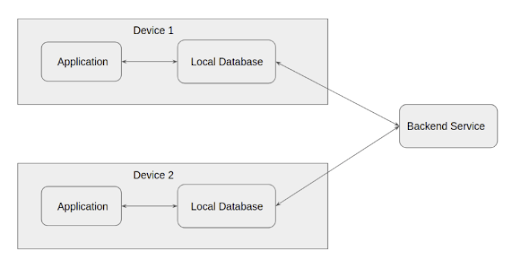
\includegraphics[width=10cm]{offline-first.png}
    \end{center}
    \caption{Simple architecture of the offline first model}
    \label{fig:offline-first}
\end{figure}

Offline first is an application development paradigm where developers ensure that the 
functionality of an app is unaffected by intermittent lack of a network connection. 
In addition offline first usually implies the ability to sync data between multiple devices
For an app to be offline first, both the code and the data required 
for it to function should not be dependent on the presence of the network.
Mobile applications do need to do something extra to make code available offline,
Web Applications however can include service workers to achieve the same.
With service workers the concern shifts to finding the safest time to update the code. 
Refer to figure \ref{fig:offline-first}.

A simple solution to making data available offline is to have a local database 
to read and write to. The database can then be replicated to and from a 
server whenever a network is available.~\cite{HasuraOfflineFirst}


\subsubsection{Push-pull replication}

RxDB can do a two-way replication(push-pull replication) with a GraphQL endpoint. 
This allows data replication from the server into the client-side database and then 
realtime query and modification.
When the user is offline, they still can use the data and later sync it with the server 
when the client is online again.

\subsubsection*{Pros}
\begin{enumerate}
    \item GraphQL-replication is faster and needs less resources.
    \item Does not need a couchdb-compliant endpoint, only a graphql-endpoint.
\end{enumerate}

\subsubsection*{Cons}
\begin{enumerate}
    \item Cannot replicate multiple databases with each other.
    \item It is assumed that the graphql-server is the single source of truth.
    \item GraphQL server has to be setup, while with couchdb-sync, the replication 
    only requires to start a server.~\cite{RxDBreplication}
\end{enumerate}


\subsubsection{Conflict resolution}
If the app can be used from multiple devices, it is possible for the user to make 
conflicting changes on different devices.

\begin{itemize}
    \item Simplest way to handle conflicts is to assume that they don’t matter and 
    users will simply correct the data later. This approach is also known as last-write-wins.
\end{itemize}

Since conflict detection and resolution is a must, there are many broad approaches, 
one of them which pouchDB uses is:

\subsubsection*{Version the objects:}

Every time a change is made a new version is created. In addition the parent version for a given 
version is also kept track. A conflict can be identified by the fact that two versions have the 
same parent. Two generic auto merge strategies are:

\begin{enumerate}
    \item \textbf{Last write wins}: Here the last revision is considered to 
    reach the server as the final value.
    \item \textbf{Merge by fields}: If the two devices modified different fields 
    of the object, it might be possible to auto merge by taking the new fields from both objects.
\end{enumerate}

In the above approach merging is done by the server and clients simply fetch the merged value. 
However if user intervention is needed to resolve a conflict, then there is a feature to merge on the client.
This will require all clients to store the version history of the document as well. A problem with this 
is that clients can independently merge the document creating new multiple merge revisions.
Clients need to handle this (For example by examining the history and ignoring one of the merge versions).

PouchDB and CouchDB handle this by using a hash of the document contents as the object version. So if two 
different devices resolve the conflict the exact same way they will end up with the exact same version id.

\subsubsection*{How are documents deleted?}

A simple way to delete objects is to have a "deleted" flag in the object. 
Merge function can then decide what to do if a deleted object has been modified. 
On the client, any object with the deleted flag set can be immediately purged as 
there will be no more updates to it. The server would need to make sure that every client has purged the object locally. 
The not so ideal but practical alternative is to periodically purge old objects.

\subsubsection*{Who uses this currently?}

PouchDB and CouchDB follow the above model. In this setup, versions are stored both on the client and 
the server. When there is a conflict a deterministic algorithm auto picks a winning version.~\cite{HasuraOfflineFirst}

\subsection{Eventual consistency via CAP theorem}

\begin{figure}[h!]
    \begin{center}
        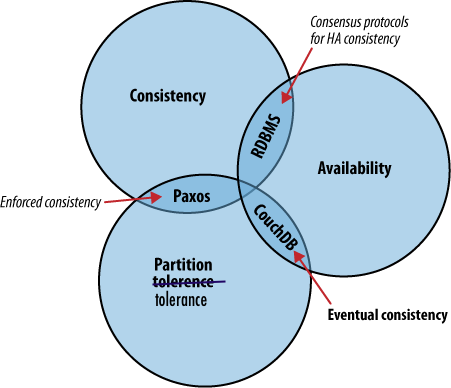
\includegraphics[width=10cm]{cap.png}
    \end{center}
    \caption{CAP Theorem. No database can offer the perfect solution for CAP.}
    \label{fig:cap}
\end{figure}

A distributed system is a system that operates robustly over a wide network. 
A particular feature of network computing is that network links can potentially 
disappear, and there are plenty of strategies for managing this type of network 
segmentation. CouchDB differs from others by accepting eventual consistency, 
as opposed to putting absolute consistency ahead of raw availability like 
RDBMS or Paxos. What these systems have in common is an awareness that data 
acts differently when many people are accessing it simultaneously. 
Their approaches differ when it comes to which aspects of consistency, 
availability, or partition tolerance they prioritize. Refer to figure \ref{fig:cap}.

The CAP theorem describes a few different strategies for distributing application 
logic across networks. CouchDB’s solution uses replication to propagate application 
changes across participating nodes. This is a fundamentally different approach from 
consensus algorithms and relational databases, which operate at different intersections 
of consistency, availability, and partition tolerance.

\begin{itemize}
    \item \textbf{Consistency}: All database clients see the same data, even with concurrent updates.
    \item \textbf{Availability}: All database clients are able to access some version of the data.
    \item \textbf{Partition tolerance}: The database can be split over multiple servers.
\end{itemize}

If availability is a priority, the clients can write data to one node of the 
database without waiting for other nodes to come into agreement. If the database 
knows how to take care of reconciling these operations between nodes, 
a sort of “eventual consistency” is achieved in exchange for high availability.

\subsubsection{MapReduce algorithm}

CouchDB uses MapReduce to compute the results of a view. MapReduce makes use of two 
functions, “map” and “reduce,” which are applied to each document in isolation. 
Being able to isolate these operations means that view computation lends itself 
to parallel and incremental computation. More important, because these functions 
produce key/value pairs, CouchDB is able to insert them into the B-tree storage engine, 
sorted by key. Lookups by key, or key range, are extremely efficient operations with a 
B-tree, described in big O notation as $O(log N)$ and $O(log N + K)$, respectively.~\cite{CouchDB}
